\documentclass[tikz,border=10pt]{standalone}
\usepackage{tikz}
\usetikzlibrary{shapes.geometric, arrows.meta, positioning, calc, fit, backgrounds, decorations.pathreplacing}

% Define colors for different components
\definecolor{backbonecolor}{RGB}{76, 175, 80}    % Green - Backbone
\definecolor{fpncolor}{RGB}{156, 39, 176}         % Purple - FPN
\definecolor{commoncolor}{RGB}{255, 193, 7}       % Amber - Common head
\definecolor{cardiocolor}{RGB}{244, 67, 54}       % Red - Cardiomegaly
\definecolor{effusioncolor}{RGB}{33, 150, 243}    % Blue - Effusion
\definecolor{latentcolor}{RGB}{233, 30, 99}       % Pink - Latent
\definecolor{decodercolor}{RGB}{255, 152, 0}      % Orange - Decoder
\definecolor{disccolor}{RGB}{158, 158, 158}       % Gray - Discriminators
\definecolor{inputcolor}{RGB}{200, 200, 200}      % Light gray - Input/Output

\tikzset{
    % Base block style
    block/.style={
        rectangle,
        draw=black,
        thick,
        minimum height=1.2cm,
        text centered,
        font=\footnotesize,
        inner sep=3pt,
    },
    % Backbone blocks
    backbone/.style={
        block,
        fill=backbonecolor!70,
        minimum width=1.5cm,
    },
    % FPN block
    fpn/.style={
        block,
        fill=fpncolor!70,
        minimum width=1.8cm,
    },
    % Conv head blocks
    convhead/.style={
        block,
        minimum width=1.6cm,
        minimum height=1cm,
    },
    % Latent block
    latent/.style={
        block,
        fill=latentcolor!70,
        minimum width=2cm,
        minimum height=1.5cm,
    },
    % Decoder blocks
    decoder/.style={
        block,
        fill=decodercolor!70,
        minimum width=1.2cm,
    },
    % Discriminator blocks
    disc/.style={
        block,
        fill=disccolor!50,
        minimum width=1.8cm,
        minimum height=0.9cm,
        rounded corners=3pt,
    },
    % Input/Output blocks
    io/.style={
        block,
        fill=inputcolor,
        minimum width=1cm,
        minimum height=2cm,
    },
    % Arrow styles
    arrow/.style={
        ->,
        >=Stealth,
        thick,
    },
    skiparrow/.style={
        ->,
        >=Stealth,
        thick,
        dashed,
        opacity=0.6,
    },
    auxarrow/.style={
        ->,
        >=Stealth,
        thick,
        dashed,
        gray,
    },
}

\begin{document}
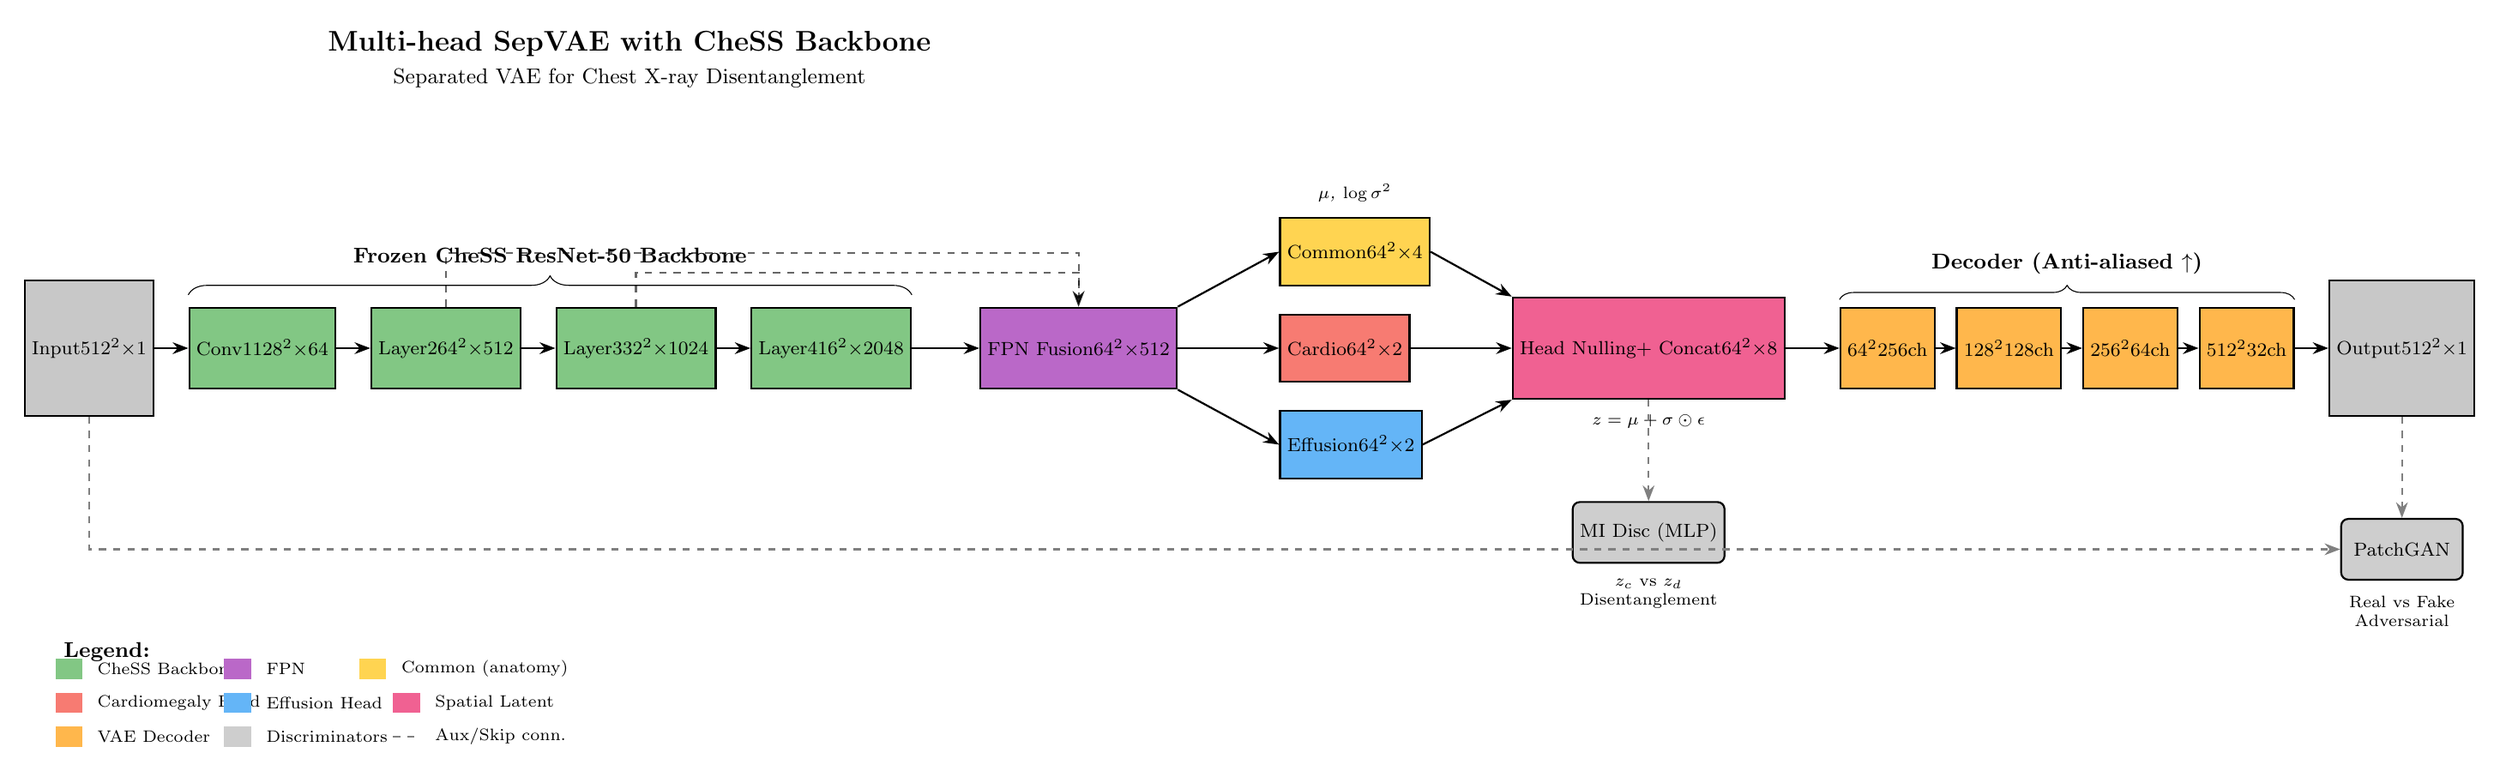
\begin{tikzpicture}[node distance=0.8cm and 0.5cm]

% =============================================================================
% TITLE
% =============================================================================
\node[font=\large\bfseries] at (8, 4.5) {Multi-head SepVAE with CheSS Backbone};
\node[font=\small] at (8, 4) {Separated VAE for Chest X-ray Disentanglement};

% =============================================================================
% INPUT
% =============================================================================
\node[io] (input) at (0, 0) {Input\\$512^2{\times}1$};

% =============================================================================
% RESNET-50 CHESS BACKBONE (FROZEN)
% =============================================================================
\node[backbone, right=of input] (conv1) {Conv1\\$128^2{\times}64$};
\node[backbone, right=of conv1] (layer2) {Layer2\\$64^2{\times}512$};
\node[backbone, right=of layer2] (layer3) {Layer3\\$32^2{\times}1024$};
\node[backbone, right=of layer3] (layer4) {Layer4\\$16^2{\times}2048$};

% Backbone label with brace
\draw[decorate, decoration={brace, amplitude=8pt, raise=5pt}]
    (conv1.north west) -- (layer4.north east)
    node[midway, above=15pt, font=\small\bfseries] {Frozen CheSS ResNet-50 Backbone};

% =============================================================================
% FEATURE PYRAMID NETWORK
% =============================================================================
\node[fpn, right=1cm of layer4] (fpn) {FPN Fusion\\$64^2{\times}512$};

% =============================================================================
% THREE PARALLEL CONV HEADS
% =============================================================================
\node[convhead, fill=commoncolor!70, above right=0.3cm and 1.5cm of fpn] (head_common) {Common\\$64^2{\times}4$};
\node[convhead, fill=cardiocolor!70, right=1.5cm of fpn] (head_cardio) {Cardio\\$64^2{\times}2$};
\node[convhead, fill=effusioncolor!70, below right=0.3cm and 1.5cm of fpn] (head_effusion) {Effusion\\$64^2{\times}2$};

% Conv heads label
\node[above=0.1cm of head_common, font=\scriptsize\itshape] {$\mu$, $\log\sigma^2$};

% =============================================================================
% HEAD NULLING & LATENT CONCATENATION
% =============================================================================
\node[latent, right=1.5cm of head_cardio] (latent) {Head Nulling\\+ Concat\\$64^2{\times}8$};

% Sampling notation
\node[below=0.1cm of latent, font=\scriptsize] {$z = \mu + \sigma \odot \epsilon$};

% =============================================================================
% DECODER (Progressive Upsampling)
% =============================================================================
\node[decoder, right=0.8cm of latent] (dec1) {$64^2$\\$256$ch};
\node[decoder, right=0.3cm of dec1] (dec2) {$128^2$\\$128$ch};
\node[decoder, right=0.3cm of dec2] (dec3) {$256^2$\\$64$ch};
\node[decoder, right=0.3cm of dec3] (dec4) {$512^2$\\$32$ch};

% Decoder label
\draw[decorate, decoration={brace, amplitude=6pt, raise=3pt}]
    (dec1.north west) -- (dec4.north east)
    node[midway, above=10pt, font=\small\bfseries] {Decoder (Anti-aliased $\uparrow$)};

% =============================================================================
% OUTPUT
% =============================================================================
\node[io, right=0.5cm of dec4] (output) {Output\\$512^2{\times}1$};

% =============================================================================
% MI DISCRIMINATOR
% =============================================================================
\node[disc, below=1.5cm of latent] (mi_disc) {MI Disc (MLP)};
\node[below=0.1cm of mi_disc, font=\scriptsize, align=center] {$z_c$ vs $z_d$\\Disentanglement};

% =============================================================================
% PATCHGAN DISCRIMINATOR
% =============================================================================
\node[disc, below=1.5cm of output] (patch_disc) {PatchGAN};
\node[below=0.1cm of patch_disc, font=\scriptsize, align=center] {Real vs Fake\\Adversarial};

% =============================================================================
% CONNECTIONS - Main Forward Path
% =============================================================================
\draw[arrow] (input) -- (conv1);
\draw[arrow] (conv1) -- (layer2);
\draw[arrow] (layer2) -- (layer3);
\draw[arrow] (layer3) -- (layer4);
\draw[arrow] (layer4) -- (fpn);

% FPN skip connections
\draw[skiparrow] (layer2.north) |- ++(0, 0.8) -| (fpn.north);
\draw[skiparrow] (layer3.north) |- ++(0, 0.5) -| (fpn.north);

% FPN to heads
\draw[arrow] (fpn) -- (head_cardio);
\draw[arrow] (fpn.north east) -- (head_common.west);
\draw[arrow] (fpn.south east) -- (head_effusion.west);

% Heads to latent
\draw[arrow] (head_common.east) -- (latent.north west);
\draw[arrow] (head_cardio) -- (latent);
\draw[arrow] (head_effusion.east) -- (latent.south west);

% Latent to decoder
\draw[arrow] (latent) -- (dec1);
\draw[arrow] (dec1) -- (dec2);
\draw[arrow] (dec2) -- (dec3);
\draw[arrow] (dec3) -- (dec4);
\draw[arrow] (dec4) -- (output);

% =============================================================================
% CONNECTIONS - Discriminators
% =============================================================================
\draw[auxarrow] (latent.south) -- (mi_disc.north);
\draw[auxarrow] (output.south) -- (patch_disc.north);
\draw[auxarrow] (input.south) |- (patch_disc.west);

% =============================================================================
% LEGEND
% =============================================================================
\begin{scope}[shift={(-0.5, -4.5)}]
    \node[font=\small\bfseries, anchor=west] at (0, 0) {Legend:};

    % Row 1
    \fill[backbonecolor!70] (0, -0.4) rectangle (0.4, -0.1);
    \node[anchor=west, font=\scriptsize] at (0.5, -0.25) {CheSS Backbone};

    \fill[fpncolor!70] (2.5, -0.4) rectangle (2.9, -0.1);
    \node[anchor=west, font=\scriptsize] at (3, -0.25) {FPN};

    \fill[commoncolor!70] (4.5, -0.4) rectangle (4.9, -0.1);
    \node[anchor=west, font=\scriptsize] at (5, -0.25) {Common (anatomy)};

    % Row 2
    \fill[cardiocolor!70] (0, -0.9) rectangle (0.4, -0.6);
    \node[anchor=west, font=\scriptsize] at (0.5, -0.75) {Cardiomegaly Head};

    \fill[effusioncolor!70] (2.5, -0.9) rectangle (2.9, -0.6);
    \node[anchor=west, font=\scriptsize] at (3, -0.75) {Effusion Head};

    \fill[latentcolor!70] (5, -0.9) rectangle (5.4, -0.6);
    \node[anchor=west, font=\scriptsize] at (5.5, -0.75) {Spatial Latent};

    % Row 3
    \fill[decodercolor!70] (0, -1.4) rectangle (0.4, -1.1);
    \node[anchor=west, font=\scriptsize] at (0.5, -1.25) {VAE Decoder};

    \fill[disccolor!50] (2.5, -1.4) rectangle (2.9, -1.1);
    \node[anchor=west, font=\scriptsize] at (3, -1.25) {Discriminators};

    \draw[dashed, thick, gray] (5, -1.25) -- (5.4, -1.25);
    \node[anchor=west, font=\scriptsize] at (5.5, -1.25) {Aux/Skip conn.};
\end{scope}

\end{tikzpicture}
\end{document}
